%%
%% Beuth Hochschule für Technik --  
%%
%% Kapitel 6 - 
%%
%%	

\newpage

[Burde]

\section{Entwurf des Reglers}

Nachdem nun die Strecke zunächst identifiziert und anschließend das Steuer- und Störverhalten simuliert wurde, soll nun der passende Regler entworfen werden. Der Regler hat dabei folgende Aufgaben: Er soll dafür sorgen, dass die Regelgeschwindigkeit des Regelkreises möglichst hoch wird, also eine möglichst kleine Anstiegszeit $t_{r}$ besitzt und er soll bleibende Regelabweichungen verhindern, also eine hohe Regelgenauigkeit vorweisen.

Die Entscheidung fällt zunächst einmal auf einen PI-Regler. Der P-Anteil sorgt für eine hohe Regelgeschwindigkeit und kompensiert somit die Trägheit des I-Anteils. Gleichzeitig sorgt jedoch der I-Anteil dafür, dass die durch den P-Anteil entstehende bleibende Regelabweichung entfernt wird. 

Um den Verstärkungsfaktor V und die Reglerzeitkonstante T optimal bestimmen zu können, wird als Entwurfsverfahren das Polkompensationsverfahren gewählt. Wie der Name schon aussagt, lassen sich bei diesem Verfahren Verzögerungsglieder aus der Strecke bzw. Messeinrichtung durch eventuelle Vorhalteglieder aus dem gewählten Regler kompensieren. Verzögerungsglieder sorgen meist für ein langsameres Ausregeln von Störgrößen und sind daher unerwünscht. Die nachfolgenden Übertragungsfunktionen vom PI-Regler sowie von der Strecke zeigen das markierte Vorhalteglied des Reglers, welches das markierte Verzögerungsglied der Strecke kompensieren soll. 

\begin{center}
$ G_{R}(s) = \dfrac{V*\textcolor{red}{(1+Ts)}}{s} $
\end{center}

\begin{center}
$ G_{S}(s) = \dfrac{1,03}{(1 + 0,003365s) * \textcolor{red}{(1 + 0,1864s)} * (1 + 2*0,98029s + (0,091032s)^{2}) }$
\end{center}

Die Zählerzeitkonstante des PI-Reglers beträgt also $ T = 0,1864[sek] $. Um den Verstärkungsfaktor des Reglers zu bestimmen, muss nun das Bodediagramm des offenen Regelkreises gezeichnet werden. Da der Aufwand dafür recht hoch ist, nutzen wir für das Verfahren der Polkompensation das Matlab-Programm \textit{polkomp}. 

Dafür muss zunächst eine maximale Überschwingweite $M_{P}$ gewählt werden. Da es dazu in der Aufgabenstellung keine konkrete Vorgabe gibt entscheiden wir uns für den gängigen Wert von 20 Prozent

\begin{center}
$ M_{p} = 0,2 $
\end{center}

Bei einer gewählten Überschwingweite zwischen 0,05 und 0,25 lässt sich mit der Formel (2.3.10a) aus dem Script  "Einführung in die Regelungstechnik" der Phasenrand $\Phi_{r}$ berechnen.

\begin{center}
$\Phi_{r}=69^\circ-106^\circ*M_{p}$
\end{center}

\begin{center}
$\Phi_{r}=69^\circ-106^\circ*0,2=47,8^\circ$
\end{center}

\newpage

Das Matlab-Programm \textit{polkomp} zeichnet uns nun das Bodediagramm des offenen Regelkreises mit einem Reglerverstärkungsfaktor von $V_{R}=1$. 

\begin{figure}[h]
	\begin{center}
		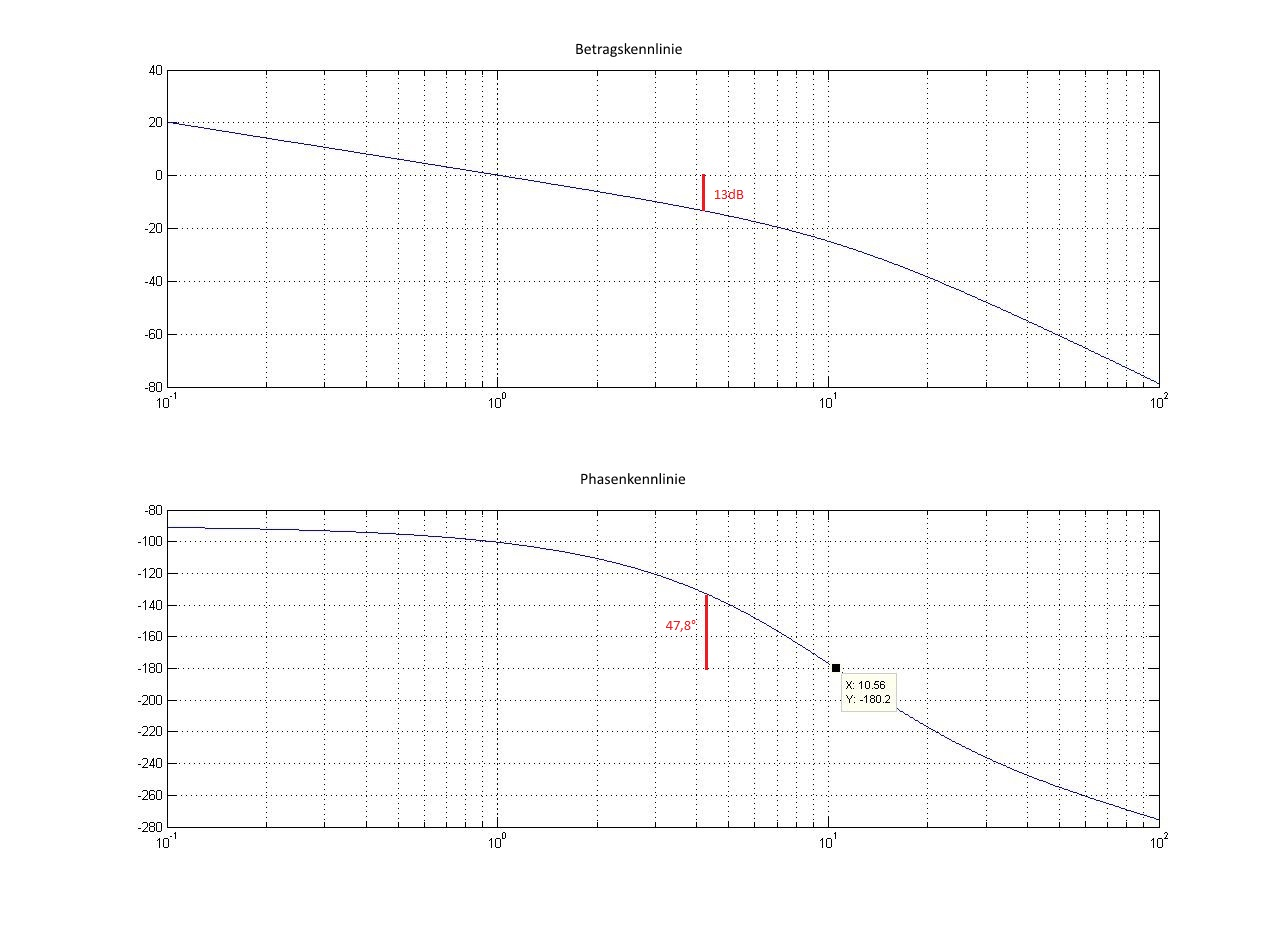
\includegraphics[scale=0.45]{bodediagramm_offener_regelkreis.jpg}
		\caption{Bodediagramm des offenen Regelkreises mit $V_{R}=1$}
       \label{bode}
	\end{center} 
\end{figure}

In Abbildung 6 ist in der Phasenkennlinie bereits der gewünschte Phasenrand von $\Phi_{r}=47,8^\circ$ eingezeichnet. Um diesen Phasenrand entstehen zu lassen, muss an dieser Stelle die Betragskennlinie durch die $0 dB$ Achse gehen. Das kann in diesem Fall mit einer Anhebung der Betragskennlinie um $13dB$ ermöglicht werden. Wählt man einen Reglerverstärkungsfaktor $V_{R}>1$ kann ein Anheben der Betragskennlinie erreicht werden. Mit der Formel (2.3.55) aus dem Script "Einführung in die Regelungstechnik" kann der Reglerverstärkungsfaktor genau berechnet werden. Nachfolgend ist die Ermittlung von $V_{R}$ per Hand dargestellt.

\begin{center}
$V_{R}=10^{\dfrac{VdB}{20dB}}$
\end{center}

\begin{center}
$V_{R}=10^{\dfrac{13dB}{20dB}}$
\end{center}

\begin{center}
$V_{R}=4,4668$
\end{center}

In der folgenden Abbildung werden die Ergebnisse der Ermittlung der Reglerparameter mit dem Matlab-Programm \textit{polkomp} abgebildet.

\newpage

\begin{figure}[h]
	\begin{center}
		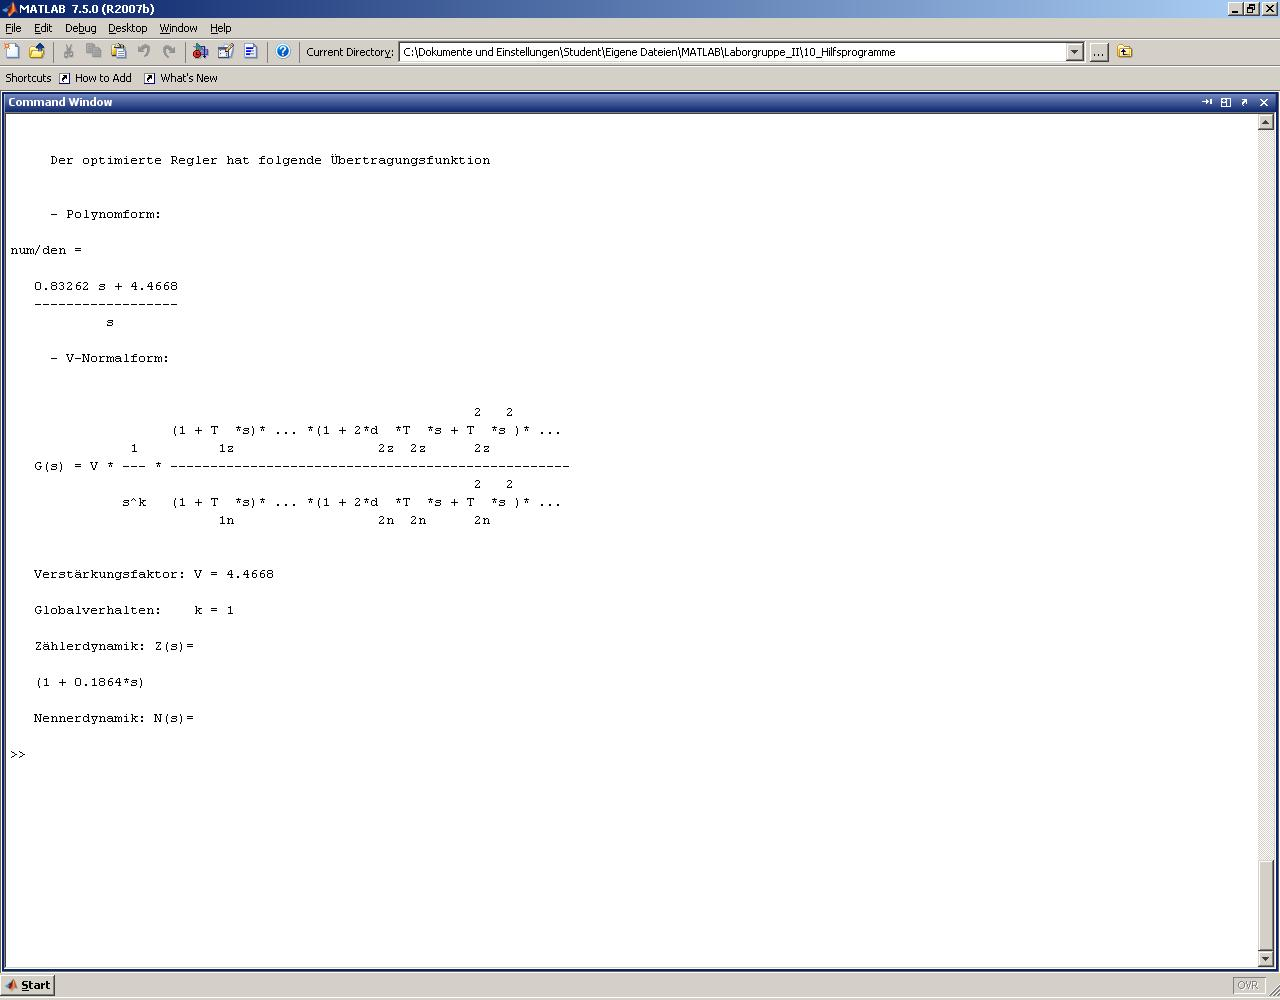
\includegraphics[scale=0.75]{regler_daten.jpg}
		\caption{Berechnete Reglerdaten mit Hilfe von \textit{polkomp}}
       \label{controllerData}
	\end{center} 
\end{figure}

Zu beachten ist hier, dass der per \textit{polkomp} ermittelte Reglerverstärkungsfaktor $V_{R}$ der gleiche ist, wie der von uns per Hand berechnete Wert. In der nächsten Abbildung wird nun die Führungssprungantwort sowie die Stellgröße des ermittelten Reglers abgebildet.

\newpage

\begin{figure}[h]
	\begin{center}
		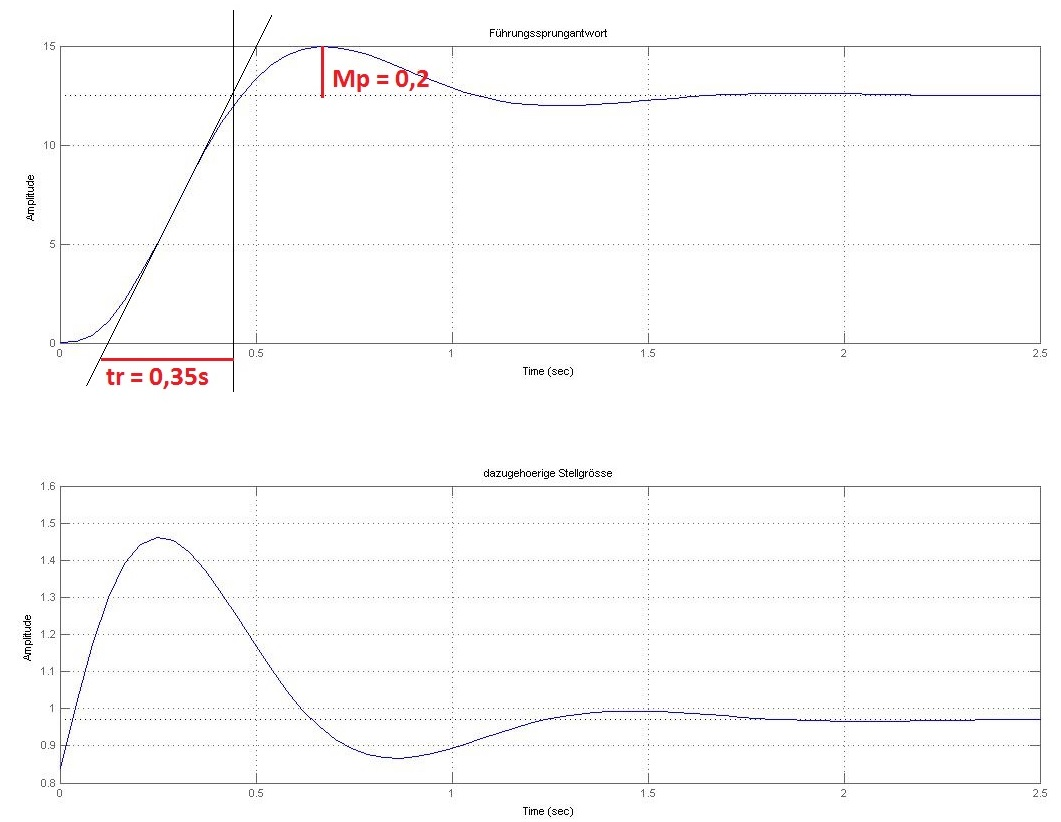
\includegraphics[scale=0.5]{pi_regler.jpg}
		\caption{Führungssprungantwort und Stellgröße des ermittelten PI-Reglers}
       \label{controller}
	\end{center} 
\end{figure}

Anhand der Führungssprungantwort ist gut zu erkennen, dass die maximal zulässige Überschwingweite $M_{p}$ von 20 Prozent nicht überschritten wird. Auch eine bleibende Regelabweichung ist nicht zu erkennen. Bei der Anstiegszeit $t_{r}$ gab es laut Aufgabenstellung zwar keine Vorgaben, es soll aber erwähnt werden, dass diese bei ungefähr $0,35s$ liegt. In dem nächsten Kapitel soll der ermittelte Regler nun in eine Simulation der Strecke integriert und das Regelverhalten erstmals getestet werden.

















